\documentclass[Main.tex]{subfiles} 
\begin{document}

\subsection{Oversigt}
Systemet er bygget op efter 3-tier arkitekturen, med de 3 lag: Presentation layer, Business logic layer og Data acces layer, som ogs� ses p� figur 3 i afsnit \textit{2.1 Systemkontekst}. Derudover har vi et fjerde lag som er selve hardwarelaget. De f�lgende afsnit vil beskrive lagene i dybden. Det er ogs� disse fire lag der ligger til grund for systemets pakker.\\
Herunder ses f�rst systemets klasser opdelt i pakker (se afsnit \textit{5.2 Arkitektursignifikante designpakker for at se hvordan pakkerne spiller sammen i en lag-opdeling. Alle diagrammerne kan ses i stor format i Bilag: Diagrammer}):
\begin{figure}[H]
\centering
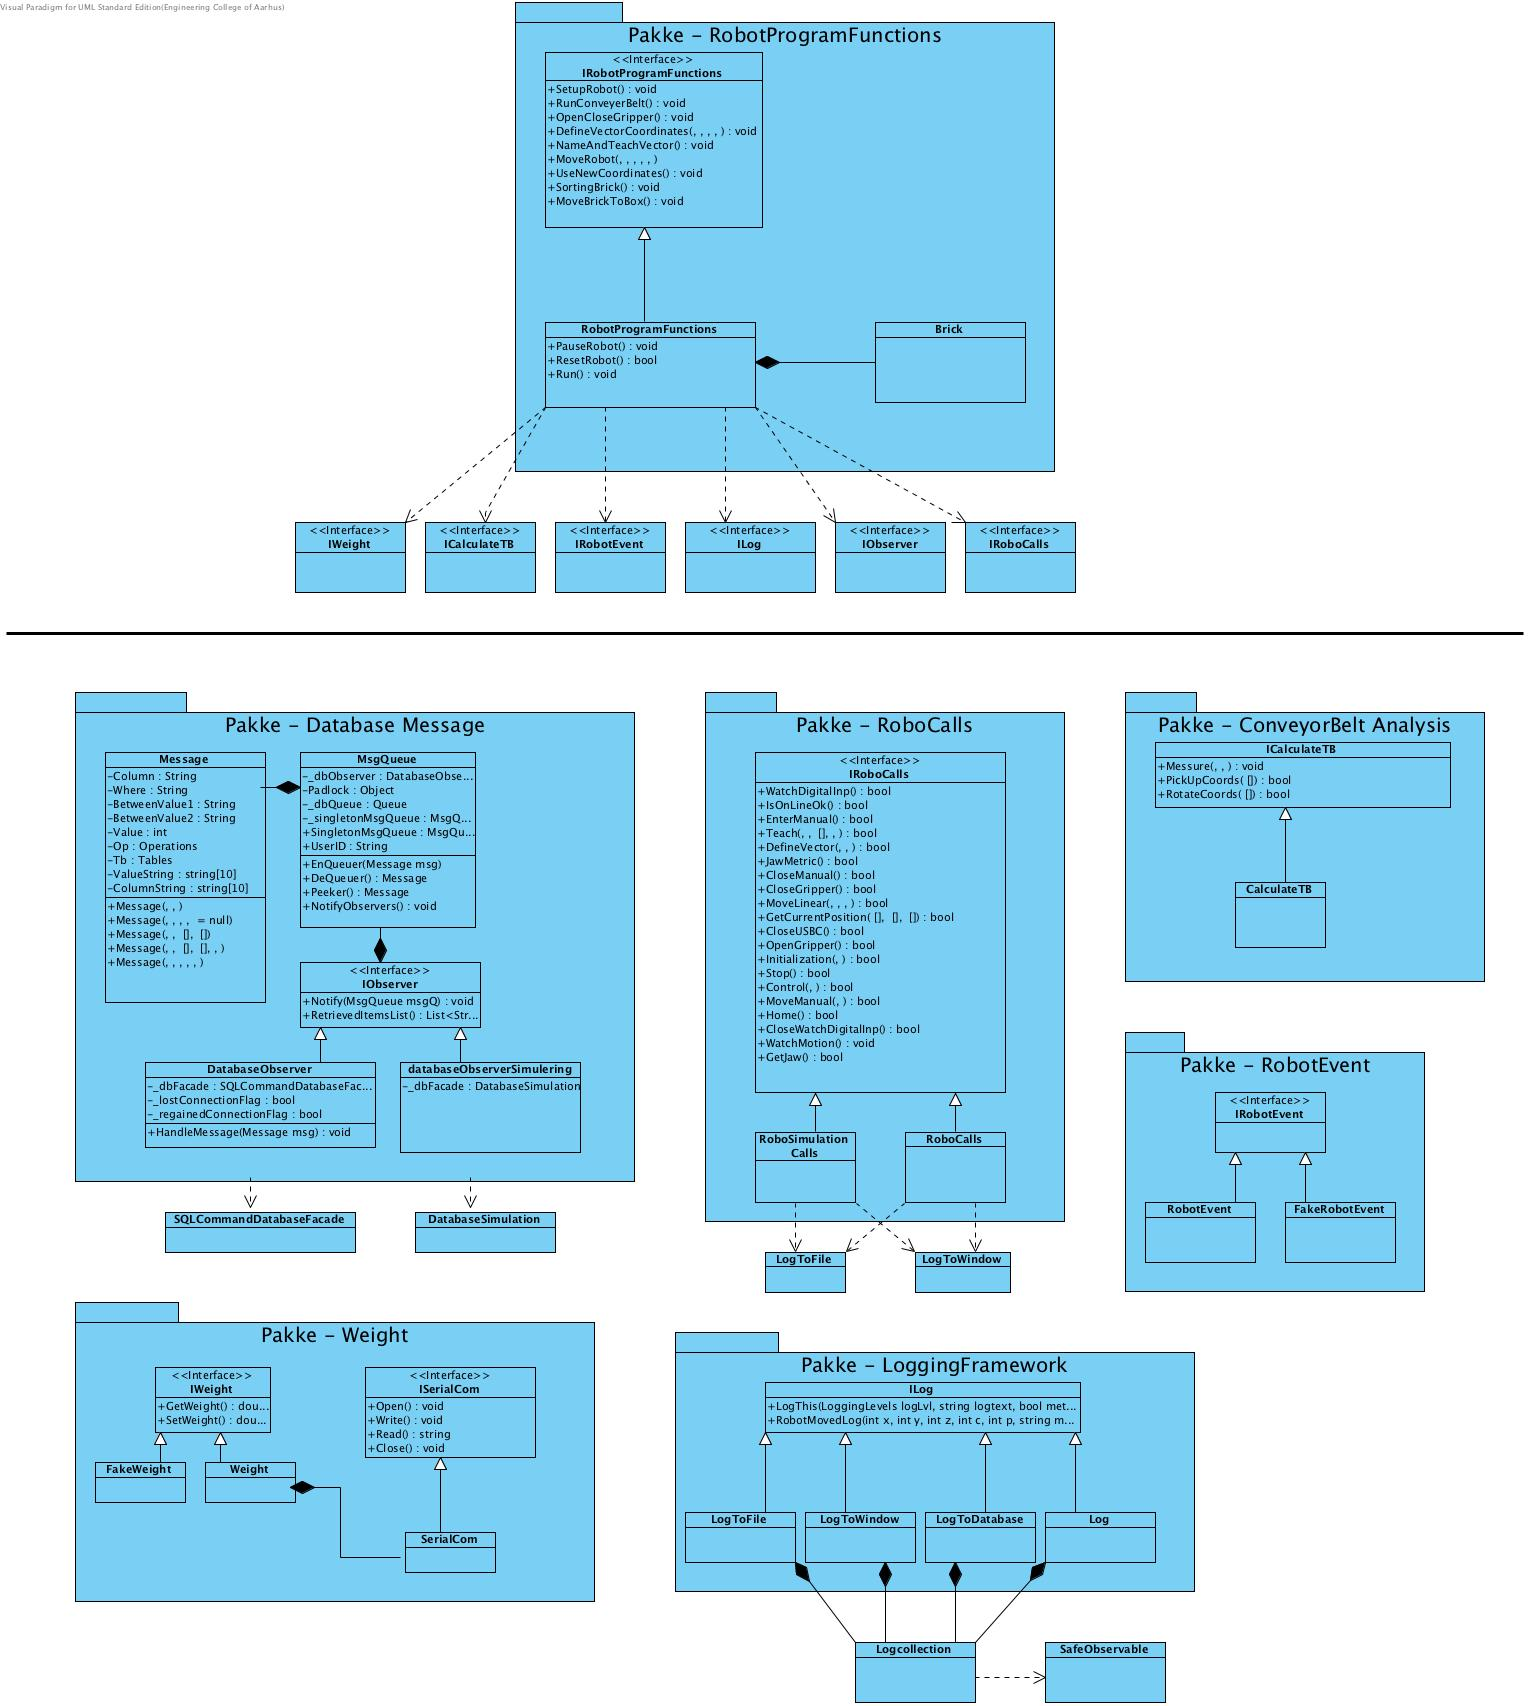
\includegraphics[scale=0.32]{Diagrammer/Klassediagrammer/Klassediagrammer/JPGFiler/Allpackages.jpg}
\caption{Hovedklasse med dets afh�ngigheder}
\end{figure}
Ovenst�ende figur viser hovedklassen (RobotProgramFunctions\footnote{Se afsnit 8.2.1 Komponent 1: Sorteringsprogram - for n�rmere information om denne klasse}, i �verste pakke), som indeholder funktioner der udg�r vores standardprogram. Nedenunder ses alle dets afh�ngigheder\footnote{Afh�ngighederne bliver ogs� brugt af andre klasser end RobotProgramFunctions.}
\begin{figure}[H]
\centering
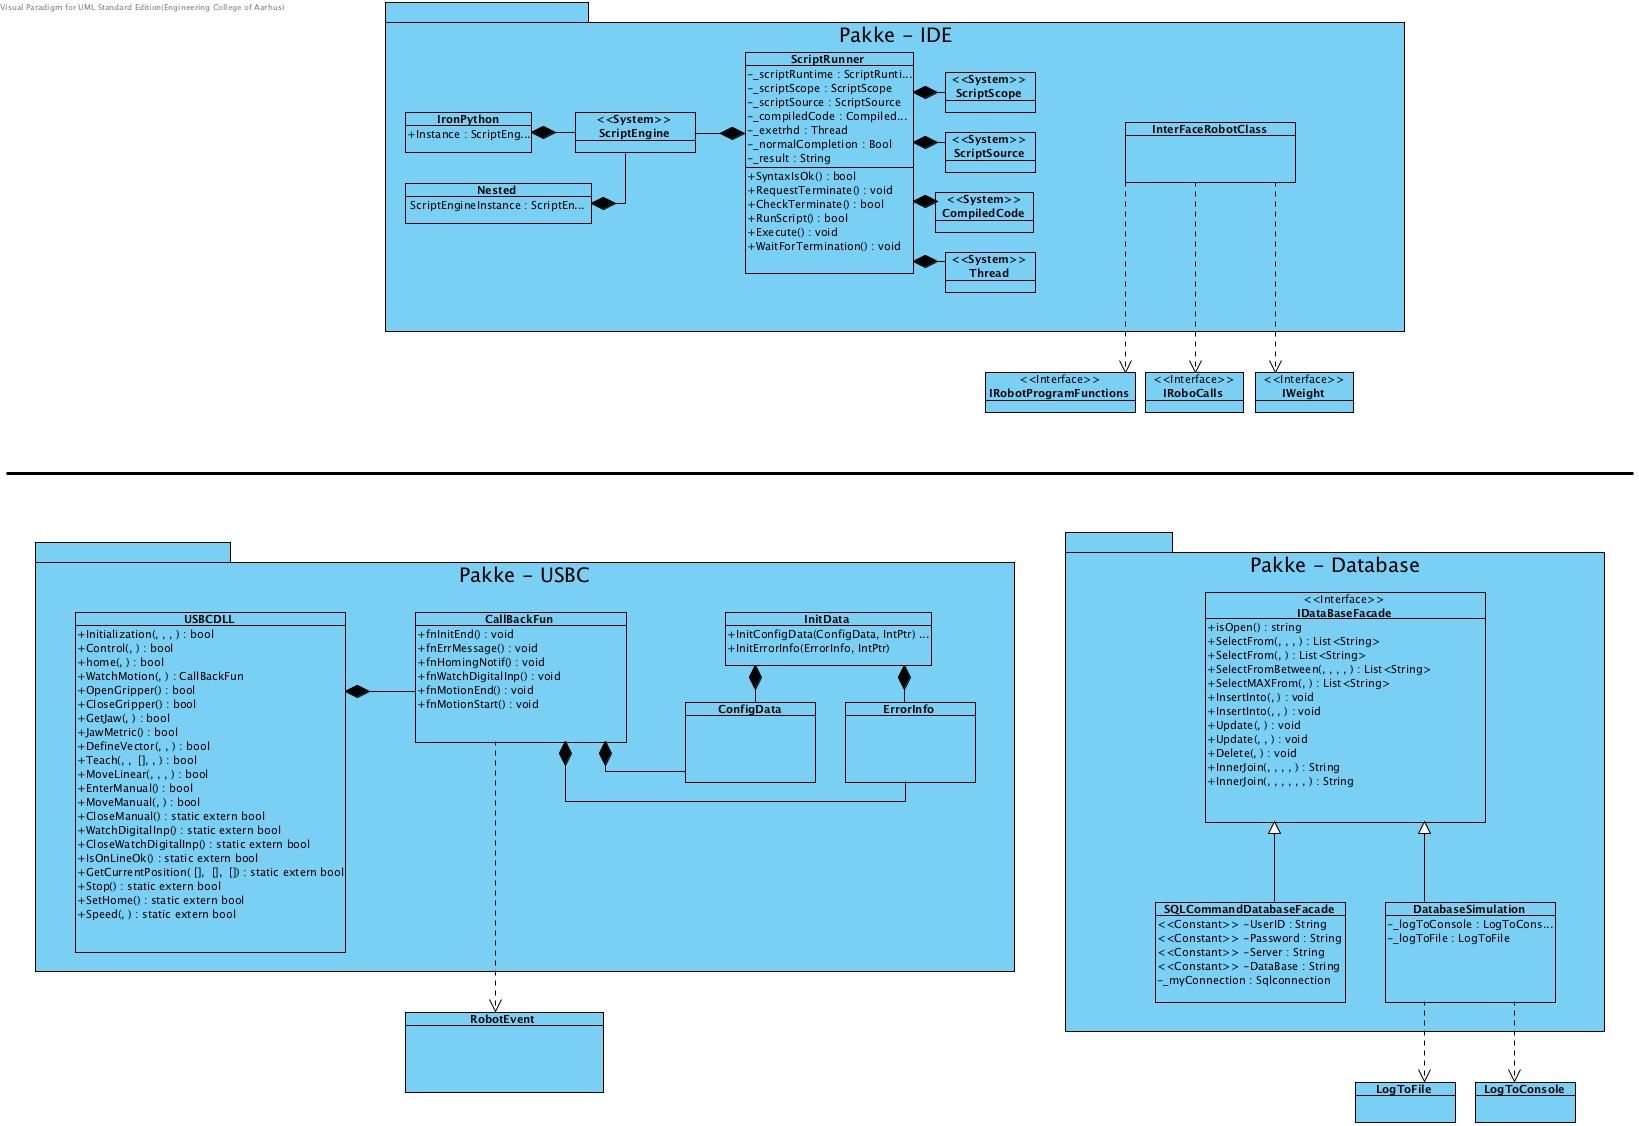
\includegraphics[scale=0.3]{Diagrammer/Klassediagrammer/Klassediagrammer/JPGFiler/Robot.jpg}
\caption{Resterende klasser}
\end{figure}
Ovenst�ende figur viser f�rst IDE'en\footnote{Se afsnit 8.2.8 Komponent8: IDE - for n�rmere information om denne klasse}, der er den anden klasse der kan tilf�je funktionalitet til robotten. De to andre pakker, benyttes b�de af standardprogrammet og IDE'en.

\end{document}